%Todo
%Table
%Colors




\documentclass[12pt,reqno,oneside]{amsbook}


%%\usepackage[english]{babel}  %Language needs to be specified for accessibility; currently this is not working well with latexml

% Math
\usepackage{amsmath, amssymb, amsthm}

% If you are including computer code the following package is useful.  It is similar to the verbatim package
\usepackage{listings} 

\usepackage{setspace}

%Graphics
\usepackage{graphicx}

% Layout
\usepackage{geometry}
\geometry{margin=1in}

% Theorem environments
\newtheorem{theorem}{Theorem}[chapter]
\newtheorem{lemma}[theorem]{Lemma}
\theoremstyle{definition}
\newtheorem{definition}[theorem]{Definition}

% Hyperref
\usepackage[pdfusetitle]{hyperref}

\begin{document}

% Title metadata.  Make changes here to fit your needs
\newcommand{\thetitle}{A Sample Thesis in Mathematics}
\title{\thetitle}
\date{\today}
\newcommand{\institution}{University of Illinois Chicago} 
\newcommand{\degree}{Doctor of Philosophy}
\newcommand{\advisor}{Prof.~Ada Lovelace}
\newcommand{\theauthor}{A.~Student}
\author{\theauthor}

\frontmatter

% Custom title page
% Take care in making substantial changes to this as it needs to still work with latexml
\begin{titlepage}
    \centering
    {\Large \institution\par}
    \vspace{2cm}
    {\Large \thetitle \par}
    \vspace{2cm}
    {\Large by\par}
    \vspace{0.5cm}
    {\Large \theauthor\par}
    \vfill
    A thesis submitted in partial fulfillment of the requirements \\
    for the degree of  \degree \\
    \vspace{0.5cm}
    Advisor: \advisor \\
    \vspace{1cm}
    \makeatletter\@date \makeatother
\end{titlepage}

\begin{abstract}
This thesis investigates XYZ. We show results about ...
\end{abstract}

\tableofcontents
\listoffigures

\mainmatter

\doublespacing %other options are \onehalfspacing or \singlespacing


\chapter{Introduction}
This is the introduction chapter. We cite some classic works \cite{Hartshorne,Mumford}.  

Lorem ipsum dolor sit amet, consectetur adipiscing elit. Morbi tincidunt nisi sed neque volutpat, et imperdiet metus congue. Donec interdum, neque at varius vehicula, elit odio tempus sapien, sed finibus lorem felis nec turpis. Aliquam erat volutpat. Mauris vehicula imperdiet erat, non aliquet magna commodo id.

Sed porttitor urna ac ipsum rhoncus, vel dictum risus commodo. Integer ultrices dui sit amet pulvinar tempor. Phasellus nec tellus eu turpis sodales accumsan. Proin ultr


\begin{theorem}\label{thm1}
This is a theorem
\end{theorem}

We reference Theorem \ref{thm1}.

\href{https://www.uic.edu}{University of Illinois Chicago}.

% JPG, JPEG, PNG will work.  PNG and SVG do not work.
\section{Motivation}


\begin{figure}\label{fig1}
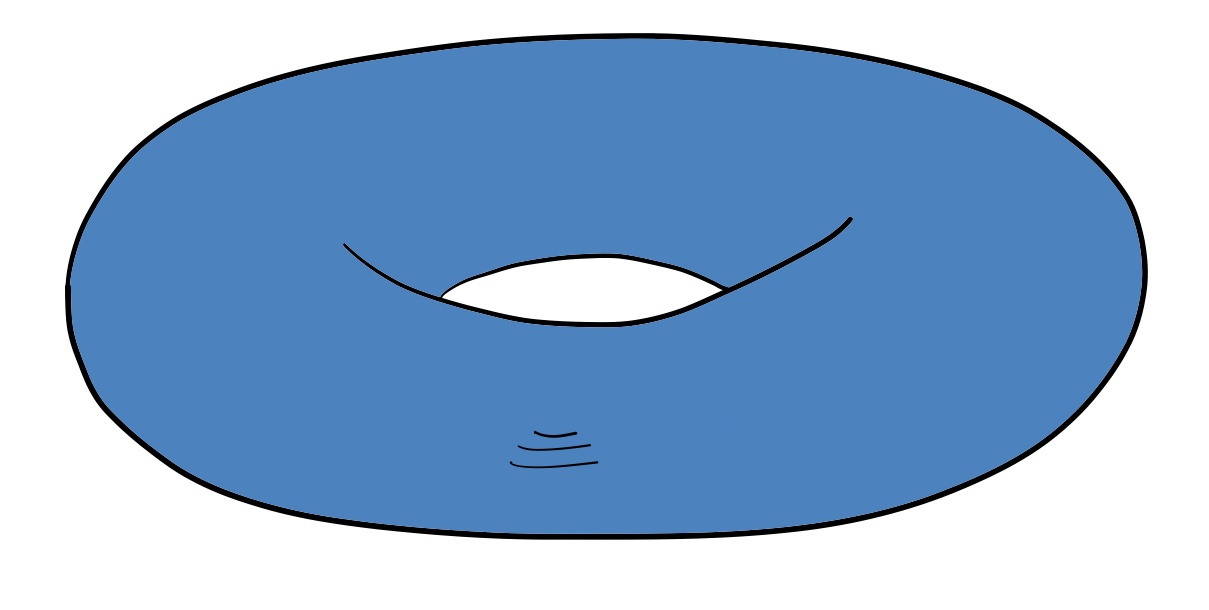
\includegraphics[alt="Description of Image that serves the same purpose",scale=0.3]{torus.jpg}
\caption{This is a torus}
\end{figure}



\begin{figure}\label{fig2}
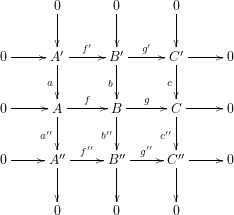
\includegraphics[alt="Description of Image that serves the same purpose",scale=0.8]{figure.png}
\caption{The Snake Lemma}
\end{figure}

%% PDF images do not work
%\begin{figure}\label{fig1}
%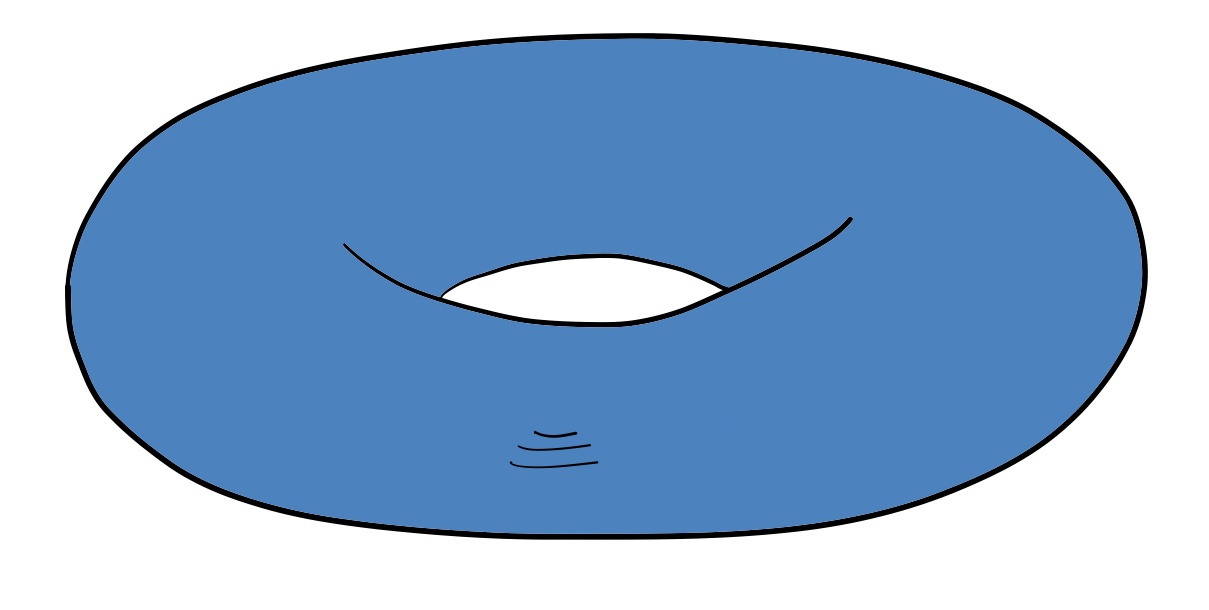
\includegraphics[alt="Description of Image that serves the same purpose",scale=0.3]{torus.pdf}
%\caption{This is a torus pdf}
%\end{figure}

\subsection{Historical context}
A brief overview of how the problem developed.
\begin{equation}\label{eq1}\int_0^1 f(x) dx = 2\end{equation}
How to solve \eqref{eq1}
\subsection{Open questions}
Some questions remain open for future work.

\section{Outline of the thesis}
We summarize the structure of the thesis.

\chapter{Background}
This chapter gives necessary background.

\section{Group theory}
\begin{definition}
A group is a set $G$ with a binary operation satisfying closure, associativity, identity, and inverses.
\end{definition}

\begin{theorem}
Every finite subgroup of the multiplicative group of a field is cyclic.
\end{theorem}

\begin{proof}
This is a standard result from algebra.
\end{proof}

\chapter{Main Results}
Here we present the main contributions of the thesis.

\section{A computer simulation}

% The following works with LaTeXml.  I consider the result accessible, but it might not be 100% WCAG compliant.
\begin{lstlisting}[basicstyle = \ttfamily\small,resetmargins=true,tabsize=5,extendedchars=false]
def factorial(n):
    """Compute the factorial of n recursively."""
    if n == 0:
        return 1
    else:
        return n * factorial(n - 1)

print(f"5! = {factorial(5)}")
\end{lstlisting}



\section{Second main result}
Another significant theorem.

\appendix
\chapter{Technical Lemmas}
Here we collect some supporting lemmas.

\begin{thebibliography}{9}


\bibitem{Hartshorne}
R.~Hartshorne, \emph{Algebraic Geometry}, Springer-Verlag, New York, 1977.

\bibitem{Mumford}
D.~Mumford, \emph{Abelian Varieties}, Oxford University Press, 1970.

\bibitem{DraismaEtAl}
J.~Draisma, E.~Horobet, G.~Ottaviani, B.~Sturmfels, and R.~R.~Thomas, 
``The Euclidean distance degree of an algebraic variety,'' 
\emph{arXiv:1309.0049} (2013).  
Available at: \href{https://arxiv.org/abs/1309.0049}{https://arxiv.org/abs/1309.0049}

\end{thebibliography}


\end{document}
